%%
%% Copyright (c) 2018 The Authors.  All Rights Reserved.
%%
%% Weitian LI, et al.
%% School of Physics and Astronomy, Shanghai Jiao Tong University,
%% Shanghai, China.
%%
%% 2018-08-23
%%

% Class options:
% - letters : for papers in the journal's Letters section (<=5 pages)
% - onecolumn : single column
% - doublespacing : double line spacing (do NOT submit in this format)
% - usenatbib : (always use this) use `natbib' package for citations
% - usegraphicx : includes the `graphicx' package
% - useAMS : support 3 upright Greek characters
% - usedcolumn : use `dcolumn' package for table column alignment

%\documentclass[letters,fleqn,usenatbib]{mnras}
\newlength{\myfigwidth}
\setlength{\myfigwidth}{\columnwidth}

%------ internal review ------
\documentclass[letters,fleqn,usenatbib,onecolumn]{mnras}
\setlength{\myfigwidth}{0.5\columnwidth}
\geometry{top=35mm,bottom=35mm,left=30mm,right=30mm}
\linespread{1.5}

\usepackage{xeCJK}
\setCJKmainfont{Noto Serif CJK SC}[BoldFont=Noto Sans CJK SC]
\setCJKsansfont{Noto Sans CJK SC}
%------ internal review ------

\usepackage{newtxtext,newtxmath}
\usepackage[T1]{fontenc}
\usepackage{ae,aecompl}

%
% Custom packages
%
\usepackage{graphicx}
\usepackage{amsmath}
\usepackage{amssymb}
\usepackage{siunitx}  % typeset units; from `texlive-science'

\graphicspath{{./}{figures/}}  % NOTE: the trailing '/' matters

\sisetup{
  range-phrase=\text{--},
  range-units=single,
  product-units=repeat,
  list-separator={, },
  list-final-separator={, and },
  separate-uncertainty=true,
}
\DeclareSIUnit\MHz{\mega\hertz}
\DeclareSIUnit\kHz{\kilo\hertz}
\DeclareSIUnit\jansky{Jy}
\DeclareSIUnit\mJy{\milli\jansky}
\DeclareSIUnit\mK{\milli\kelvin}

\def\sectionautorefname{Section}
\def\subsectionautorefname{Section}
\def\figureautorefname{Fig.}
\def\tableautorefname{Table}

%
% Custom commands
%
\newcommand{\R}[1]{\mathrm{#1}}
\newcommand{\B}[1]{\mathbfit{#1}}
\newcommand{\M}[1]{\mathbfss{#1}}


%%======================================================================
%% Title page
%%

%      ............................................. (<=45 chars)
\title[EoR Separation with CDAE]{%
  A Deep-learning-based Method to Separate the EoR Signal
  Using the Convolutional Denoising Autoencoder
}

% If you need two or more lines of authors, add an extra line using \newauthor
\author[Li~et~al.]{%
Weitian Li,$^{1}$\thanks{E-mail:
  \href{mailto:liweitianux@sjtu.edu.cn}{liweitianux@sjtu.edu.cn} (WL);
  \href{mailto:hgxu@sjtu.edu.cn}{hgxu@sjtu.edu.cn} (HX)}
Haiguang Xu,$^{1,2}$\footnotemark[1]
Zhixian Ma,$^{3}$
Ruimin Zhu,$^{4}$
Dan Hu,$^{1}$
Zhenghao Zhu,$^{1}$
\newauthor  % start on a new line
Chenxi Shan,$^{1}$
Jie Zhu$^{3}$
and
Xiang-Ping Wu$^{5}$
\\
% List of institutions
$^{1}${School of Physics and Astronomy,
  Shanghai Jiao Tong University,
  800 Dongchuan Road, Shanghai 200240, China} \\
$^{2}${Tsung-Dao Lee Institute / IFSA Collaborative Innovation Center,
  Shanghai Jiao Tong University,
  800 Dongchuan Road, Shanghai 200240, China} \\
$^{3}${Department of Electronic Engineering,
  Shanghai Jiao Tong University,
  800 Dongchuan Road, Shanghai 200240, China} \\
$^{4}${Department of Statistics,
  Northwestern University,
  2006 Sheridan Road, Evanston, IL 60208, US} \\
$^{5}${National Astronomical Observatories,
  Chinese Academy of Sciences,
  20A Datun Road, Beijing 100012, China}
}

% These dates will be filled out by the publisher
\date{Accepted XXX. Received YYY; in original form ZZZ}

% Enter the current year, for the copyright statements etc.
\pubyear{2018}

% Don't change these lines
\begin{document}
\label{firstpage}
\pagerange{\pageref{firstpage}--\pageref{lastpage}}
\maketitle

%
% Abstract
% (<=200 words for Letters)
%
\begin{abstract}
When applying the foreground removal methods to uncover the extremely
faint signal from the epoch of reionization (EoR), the foreground spectra
are assumed to be smooth.
This assumption, however, can be seriously violated since the rapid
fluctuations of residual foreground sources along the frequency
dimension, which are caused by the frequency-dependent beam effects of
the interferometers, usually cannot be avoided in practice.
To address this issue, we propose a novel deep-learning-based method
that uses a convolutional denoising autoencoder (CDAE) consisting of
a 4-layer encoder, a 4-layer decoder, and one output layer.
After being trained on the simulated SKA images with realistic beam
effects considered,
the CDAE achieves excellent performance as the correlation coefficient
between the reconstructed and input EoR signal reaches
$\rho_{\R{CDAE}} = \num{0.969 +- 0.020}$.
In comparison, the polynomial fitting method fails to distinguish the
EoR signal from the fluctuations caused by the beam effects, leading to
an unacceptable result ($\rho_{\R{poly}} = \num{0.241 +- 0.103}$).
{\color{cyan}%
Owing to the architecture of stacking multiple convolutional layers,
the CDAE hierarchically learns the subtle features of the EoR signal,
which is flexible and powerful.
In conclusion, the CDAE can overcome the frequency-dependent beam effects
and accurately separate the EoR signal, exhibiting the great potential
of deep learning methods in future EoR experiments.} % color
\end{abstract}

% Select between one and six entries from the list of approved keywords.
% Don't make up new ones.
% https://academic.oup.com/DocumentLibrary/mnras/keywords.pdf
\begin{keywords}
methods: data analysis --
techniques: interferometric --
dark ages, reionization, first stars --
radio continuum: general
\end{keywords}


%%======================================================================
%% Paper body
%%

\section{Introduction}
\label{sec:intro}

The \SI{21}{\cm} line emission of neutral hydrogen from the
epoch of reionization (EoR), a period of the early Universe
($z \sim \numrange{6}{15}$) that is still poorly understood, is regarded
as a decisive probe to directly explore the cosmic reionization
\citep[see][for reviews]{furlanetto2006rev,furlanetto2016rev}.
To detect the \SI{21}{\cm} signal, which is believed to have been
redshifted to the frequencies below \SI{200}{\MHz}, low-frequency
radio interferometers have been built or under construction, including
21CMA \citep{zheng2016}, GMRT \citep{paciga2011}, MWA \citep{tingay2013},
LOFAR \citep{vanHaarlem2013}, PAPER \citep{parsons2010},
HERA \citep{deboer2017}, and SKA \citep{koopmans2015rev}.
The observational challenges, however, are immense due to a variety of
complicated instrumental effects, ionospheric distortions, radio frequency
interference, and the strong astronomical foreground contamination that
overwhelms the EoR signal by about \numrange{4}{5} orders of magnitude
(see \citealt{morales2010rev} for a review).
Fortunately, in the frequency dimension the foreground contamination
is expected to be intrinsically smooth, while the EoR signal fluctuates
rapidly on $\lesssim \si{\MHz}$ scales.
This difference is the key characteristic exploited by many
foreground removal methods in order to uncover the faint EoR signal,
including parametric fitting approaches
\citep[e.g.,][]{wang2006,liu2009fgrm,wang2013}
and non-parametric approaches
\citep[e.g.,][]{harker2009,chapman2013,mertens2018}.

However, the smoothness of the foreground spectra can be destroyed by
the frequency-dependent beam effects, i.e., the variation of the point
spread function (PSF) with frequencies that cannot be perfectly
calibrated \citep{liu2009ps}.
Because of the incomplete $uv$ coverage,
the PSF has a complicated profile consisting of a narrow peaky main lobe
and a multitude of jagged side lobes with relative amplitudes of about
\numrange{0.1}{1} per cent that extend beyond the field of view (FoV)
\citep[e.g.,][figures 1 and 3]{liu2009ps}.
{\color{cyan}%
A source that is unresolved or mis-subtracted (e.g., due to the limited
FoV) during the CLEAN process leaves catastrophic residuals,
the locations of which change with the frequency since the angular
position of a PSF side lobe is inversely proportional to the frequency.}
These effects lead to complicated residuals fluctuating along the
frequency dimension, which cannot be correctly separated from the EoR
signal by using the standard foreground removal methods that rely on
the smoothness of the foreground spectra.

Given the complicated profiles and frequency-dependent variations of
the PSF, it would be difficult to craft a practicable model for most,
if not all, existing foreground removal methods to overcome the beam
effects, even at the cost of extensive computation burden
\citep[e.g.,][]{lochner2015,vafaeiSadr2018}.
{\color{cyan}%
Thus deep-learning-based methods, which can distill knowledge from the
data and automatically refine the model, seem more feasible and
appealing \citep[e.g.,][]{herbel2018,vafaeiSadr2018}.}
In recent years, the deep learning algorithms have seen prosperous
developments and have brought breakthroughs into many fields
(see \citealt{lecun2015} for a recent review).
Among various deep learning algorithms, the convolutional denoising
autoencoder (CDAE) and its variants are flexible and powerful in
learning subtle and complicated features from the data and have been
successfully applied to
weak gravitational wave signal denoising \citep[e.g.,][]{shen2017},
monaural audio source separation \citep[e.g.,][]{grais2017}, and so on.
{\color{cyan}%
These applications have demonstrated the abilities of the CDAE in
extracting weak signals from highly temporal-variable data.
We expect that the CDAE is promising to accurately separate
the EoR signal;
although the signal-to-noise ratio in the EoR detection is much lower
than in existing applications, the EoR signal and foreground emission
as well as the beam effects are stationary or semi-stationary.} % color

In this paper, a novel deep-learning-based method that uses a CDAE
is proposed to tackle the intricate frequency-dependent beam effects
and to separate the EoR signal along the frequency dimension.
In \autoref{sec:method}, we briefly introduce the CDAE and elaborate
the proposed method.
In \autoref{sec:experiments}, we demonstrate the performance of the
CDAE by applying it to the simulated SKA images.
We discuss the method and carry out a comparison to the standard
polynomial fitting method in \autoref{sec:discussions}.
Finally, we summarize our work in \autoref{sec:summary}.
The implementation code and data are made public at
\url{https://github.com/lwieitianux/cdae-eor}.


%%======================================================================
\section{Methodology}
\label{sec:method}

%%----------------------------------------------------------------------
\subsection{Convolutional denoising autoencoder}
\label{sec:cdae}

An autoencoder is composed of an encoder and a decoder, which can be
characterized by the functions $f(\cdot)$ and $g(\cdot)$, respectively.
The encoder maps the input $\B{x}$ to an internal code $\B{h}$, i.e.,
$\B{h} = f(\B{x})$, and the decoder tries to reconstruct the wanted
signal from the code $\B{h}$, i.e., $\B{r} = g(\B{h})$, where $\B{x}$,
$\B{h}$, and $\B{r}$ are all vectors (see also \autoref{sec:architecture}).
By placing constraints (e.g., dimensionality, sparsity, etc.\@) on the
internal code $\B{h}$ and training the autoencoder to minimise the
loss $L(\B{r}, \B{x})$, which quantifies the difference between the
reconstruction $\B{r}$ and the input $\B{x}$, the autoencoder tries to
learn the codes that effectively represent the input data
\citep[e.g.,][chapter 14]{goodfellow2016}.
{\color{cyan}%
When the autoencoder is trained to map the noisy input data to the
corresponding noise-free signal, the learned features will be robust to
the noise, and the trained autoencoder can thus reconstruct the denoised
signal from the noisy input data, hence the `denoising autoencoder'
\citep{vincent2008,vincent2010}.
By introducing the architecture of stacking multiple convolutional
layers, one of the major innovations of the convolutional neural network,
into the denoising autoencoder, the CDAE gains the benefits of
hierarchically learning the more and more sophisticated features from
the data, which is a versatile technique that contributes to the great
success of the convolutional neural network \citep{du2017}.} % color

In the EoR detection task, the foreground contamination can be regarded
as strong noise that suppress the EoR signal.
Therefore, the CDAE is employed to learn the features of the EoR signal
$\B{r}_{\R{EoR}}$ from the input ($\B{x} = \B{x}_{\R{EoR}} + \B{x}_{\R{fg}}$)
and to obtain the reconstructed signal $\B{r}_{\R{EoR}}$ that is
expected to be as close to the input $\B{x}_{\R{EoR}}$ as possible.


%%----------------------------------------------------------------------
\subsection{Network architecture}
\label{sec:architecture}

We follow common practices to build the CDAE architecture
\citep[e.g.,][]{suganuma2018,geron2017}.
The encoder part is symmetric to the decoder part, and both of them
use the exponential linear unit (ELU) as the activation function
\citep{clevert2016},
while the output layer uses the hyperbolic tangent function (i.e., tanh)
as the activation function (see also \autoref{sec:preprocessing}).
The batch normalisation is applied to all layers except for the output
layer to improve the training process as well as to act as a regularizer
to prevent overfitting \citep{ioffe2015}.
The filters are vectors of length 3 [即向量长度,无单位] in all layers,
since each of the CDAE's input $\B{x}$ is the emission of one sky pixel,
i.e., a vector of length $n_f$ with $n_f$ being the number of frequency
channels in the image cube (see also \autoref{sec:simulation}).

We have evaluated the performance of multiple CDAE architectures, each
containing a different number of layers and filters.
The simplest one with sufficiently good performance is selected,
which consists of a 4-layer encoder with $(32,64,64,32)$ filters,
a 4-layer decoder with $(32,64,64,32)$ filters, and one output layer,
as shown in \autoref{fig:network}.

\begin{figure}
  \centering
  \includegraphics[width=0.8\myfigwidth]{network-crop}
  \caption{\label{fig:network}%
    The network architecture of the proposed CDAE, consisting of a
    4-layer encoder (the orange boxes), a 4-layer decoder (the blue
    boxes), and one output layer (the green box).
    The layers in the encoder and decoder use the ELU activation
    function and batch normalisation (BN), while the output layer uses
    the `tanh' activation function.
    All filters are vectors of length 3 and the number of filters in
    each layer is marked in the braces.
  }
\end{figure}


%%----------------------------------------------------------------------
\subsection{Training and evaluation}
\label{sec:train-eval}

The CDAE is initialised by the He uniform initialiser \citep{he2015}
and is trained using the Adam optimisation method \citep{kingma2015}.
The loss, which describes the difference between the reconstructed EoR
signal $\B{r}_{\R{EoR}}$ and the input EoR signal $\B{x}_{\R{EoR}}$
(see \autoref{sec:simulation}),
is calculated as the mean squared error (MSE), i.e.,
\begin{equation}
  \label{eq:loss}
  L = \frac{1}{N} \sum_{i=1}^{N}
    \left[ \B{r}_{\R{EoR}}^{(i)} - \B{x}_{\R{EoR}}^{(i)} \right]^T
    \left[ \B{r}_{\R{EoR}}^{(i)} - \B{x}_{\R{EoR}}^{(i)} \right],
\end{equation}
where $N$ is the number of data points in the training dataset
(see \autoref{sec:training}).
By being trained to minimise the loss, the CDAE gains the ability to
reconstruct the EoR signal from the input data
($\B{x} = \B{x}_{\R{EoR}} + \B{x}_{\R{fg}}$).

To evaluate the performance of the CDAE in separating the EoR signal,
the commonly used Pearson's correlation coefficient
\citep[e.g.,][]{harker2009,chapman2013}
is adopted to measure the similarity between the reconstructed EoR
signal $\B{r}_{\R{EoR}}$ and the input EoR signal $\B{x}_{\R{EoR}}$:
\begin{equation}
  \label{eq:corrcoef}
  \rho(\B{r}_{\R{EoR}}, \B{x}_{\R{EoR}}) =
    \frac{\sum_{j=1}^{n}(r_{\R{EoR},j} - \bar{r}_{\R{EoR}})
      (x_{\R{EoR},j} - \bar{x}_{\R{EoR}})}{
        \sqrt{\sum_{j=1}^{n}(r_{\R{EoR},j} - \bar{r}_{\R{EoR}})^2
          \sum_{j=1}^{n}(x_{\R{EoR},j} - \bar{x}_{\R{EoR}})^2}
    },
\end{equation}
where $n$ is the length of the signals,
and $\bar{r}_{\R{EoR}}$ and $\bar{x}_{\R{EoR}}$ represent the mean values.
The closer the correlation coefficient is to one, the better the
performance of separation.


%%======================================================================
\section{Experiments}
\label{sec:experiments}

%%----------------------------------------------------------------------
\subsection{Simulation of the SKA images}
\label{sec:simulation}

We carry out end-to-end simulations to generate the SKA images to
train the proposed CDAE and evaluate its performance.
We choose the \SI{8}{\MHz} frequency band centred at \SI{158}{\MHz} as
an example, which is divided into $n_f = 101$ channels with a resolution
of \SI{80}{\kHz}.
Following the approach described in detail in our previous works
\citep{wang2010,wang2013}, we simulate the sky maps of the foreground
emission contributed by the Galactic synchrotron and free-free
emissions, extragalactic point sources (the bright ones with a
\SI{158}{\MHz} flux density $S_{158} > \SI{10}{\mJy}$ are assumed to
have been removed; e.g., \citealt{liu2009ps}), and radio haloes.
The sky maps of the EoR signal are created using the `faint galaxies'
data released by the Evolution Of 21~cm Structure project
(EOS; \citealt{mesinger2016}).
The simulated sky maps cover a sky area of \SI{10 x 10}{\degree} and are
pixelised into \num{1800 x 1800} with a pixel size of \SI{20}{\arcsecond}.

To fully take into account the frequency-dependent beam effects,
the SKA1-Low layout configuration\footnote{\raggedright%
  SKA1-Low layout:
  \url{https://astronomers.skatelescope.org/wp-content/uploads/2016/09/SKA-TEL-SKO-0000422_02_SKA1_LowConfigurationCoordinates-1.pdf}}
is employed in the \textsc{oskar}\footnote{%
  OSKAR: \url{https://github.com/OxfordSKA/OSKAR} (version 2.7.0)}
\citep{mort2010} to simulate observations for the sky maps,
yielding the visibility data, from which the observed images are created
by the \textsc{wsclean}\footnote{%
  WSClean: \url{https://sourceforge.net/p/wsclean} (version 2.5)}
imager \citep{offringa2014} with the natural weighting and baseline
range of \numrange{30}{1000} wavelengths in order to emphasise the
faint diffuse EoR signal.
The created images are cropped to keep only the central
\SI{2 x 2}{\degree} regions (i.e., \num{360 x 360} pixels) for the sake
of the best imaging quality.
Therefore, we obtain two image cubes of the size \num{360 x 360 x 101}
for the EoR signal ($C_{\R{EoR}}$) and the foreground emission
($C_{\R{fg}}$), respectively.
An example spectrum and the corresponding differential spectrum for
the foreground emission are shown in \autoref{fig:simudata}.
It is clearly shown that, compared with the original foreground spectrum
(the top panel),
{\color{cyan}%
the smoothness of the foreground spectrum is seriously damaged by the
jagged fluctuations with strength of about \SI{10}{\mK}
(the bottom panel),
resulting from the frequency-dependent beam effects introduced by the
interferometric observation.}

\begin{figure}
  \centering
  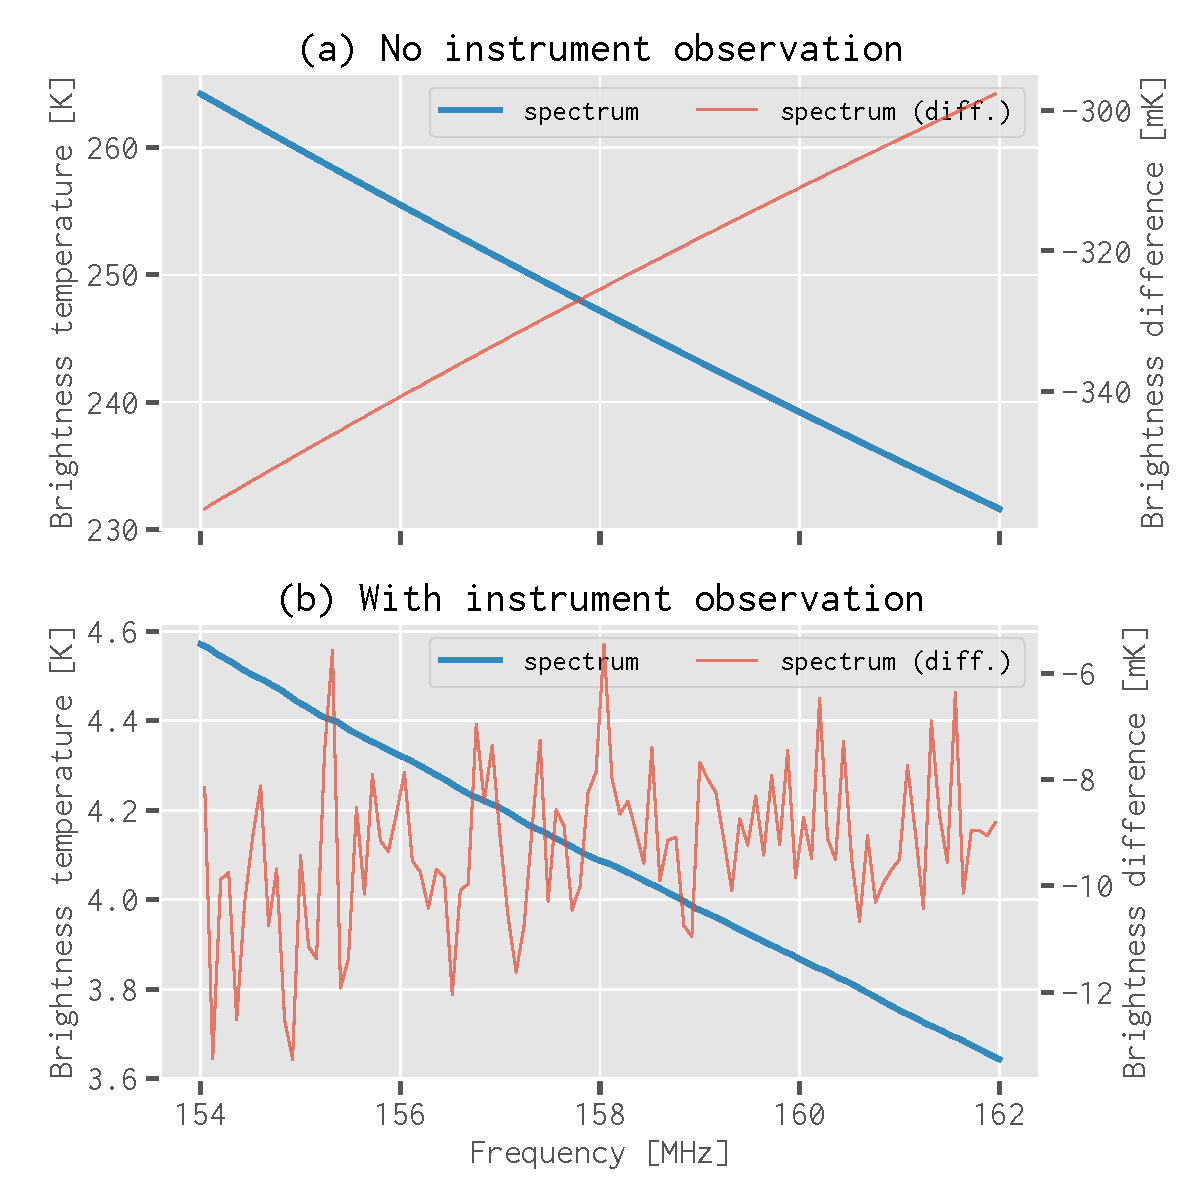
\includegraphics[width=\myfigwidth]{simudata}
  \caption{\label{fig:simudata}%
    Example spectra (the bold blue lines) and the corresponding
    differential spectra (the thin red lines) for the foreground
    emission.
    The top and bottom panels show the cases without and with
    instrument observation, respectively.
  }
\end{figure}


%%----------------------------------------------------------------------
\subsection{Data preprocessing}
\label{sec:preprocessing}

{\color{cyan}%
The dataset $S = \{(\B{x}, \B{x}_{\R{EoR}})\}$ for the CDAE is derived
from the simulated image cubes (i.e., $C_{\R{EoR}}$ and $C_{\R{fg}}$),
with each of the data point $(\B{x}, \B{x}_{\R{EoR}})$ representing
the total emission and the EoR signal of one pixel in the image cubes,
respectively, i.e., $\B{x} = \B{x}_{\R{EoR}} + \B{x}_{\R{fg}}$.
The dataset thus consists of $N = \num{360x360} = \num{129600}$ data points.}

For the input data $X = \{\B{x}\}$, we propose to apply the
Fourier Transform (FT) along the frequency dimension,
which makes the EoR signal more distinguishable from the
foreground emission and thus easier to be learned by the CDAE
(a comparison with the results derived without applying the FT is
presented in \autoref{sec:why-ft}).
The Blackman-Nuttall window function is applied to suppress the
FT side-lobes caused by the sharp discontinuities at both ends
of the finite frequency band \citep[e.g.,][]{chapman2016}.
It is sufficient to keep only half the Fourier coefficients because
$\B{x}$ is real, thus $\B{x}$ of length $n_f = 101$ is transformed to
be 51 complex Fourier coefficients,
{\color{cyan}%
among which the $n_{\R{ex}}$
coefficients of the lowest Fourier frequencies are excised since they
are mostly contributed by the spectral-smooth foreground emission.
We adopt $n_{\R{ex}} = 6$ to achieve a trade-off between the benefit of
foreground suppression and the loss of data.
The real and imaginary parts of the remaining 45 complex coefficients
are then concatenated into a new real vector of length 90, as the CDAE
requires real data.}
Finally, the data are zero-centred and normalised to have unit variance.

The preprocessing steps for the input EoR signal $X_{\R{EoR}}$ are
basically the same except for minor adjustments.
After applying the FT, excising the $n_{\R{ex}}$ lowest Fourier
components, and concatenating the real and imaginary parts,
the data elements that have a value less than the 1$^{\R{st}}$
percentile or greater than the 99$^{\R{th}}$ percentile are truncated,
{\color{cyan}%
in order to prevent the possible outliers hindering the training of
the CDAE.
Finally, the value range of the data is scaled to be $[-1, 1]$ by
dividing by the maximum absolute value,
which allows to use the `tanh' activation function with the same value
range in the output layer of the CDAE (\autoref{sec:architecture}).}


%%----------------------------------------------------------------------
\subsection{Training}
\label{sec:training}

The preprocessed dataset is randomly partitioned into the
training set ($S_{\R{tr}}$), validation set ($S_{\R{val}}$),
and test set ($S_{\R{test}}$) that account for
60, 20, and 20 per cent of the whole dataset, respectively.
The training set is used to train the parameters of the CDAE by
minimising the loss,
the validation set helps to determine the hyperparameters (e.g., the
number of layers and filters, the choice of the loss function),
while the test set is only employed to evaluate the performance of the
trained CDAE.
[如此划分和使用 training/validation/test 数据集是机器学习的惯例;
老马的文章在 pre-training 和 fine-tuning 两个阶段都使用了
validation 数据集,用来说明网络训练效果是否良好,所选网络架构是否合理;
与此处的描述是一致的。]

We implement the proposed CDAE using the popular \textsc{Keras}\footnote{%
  Keras: \url{https://keras.io} (version 2.2.0)}
framework \citep{keras} with the \textsc{TensorFlow}\footnote{%
TensorFlow: \url{https://www.tensorflow.org} (version 1.4.1)}
back end \citep{tensorflow}.
The parameters of the Adam optimisation method are set to the default
values, i.e., learning rate being $\alpha = 0.001$, and
exponential decay rates for the first and second moment estimates being
$\beta_1 = 0.9$ and $\beta_2 = 0.999$, respectively \citep{kingma2015}.
The CDAE is trained on the training set ($S_{\R{tr}}$) with a batch size
of 100 for 100 epochs until the training loss converges.


%%----------------------------------------------------------------------
\subsection{Results}
\label{sec:results}

The training and validation losses together with the evaluation index
(i.e., the correlation coefficient) calculated on the validation set
($S_{\R{val}}$) during the training phase are shown in \autoref{fig:train}.
The steadily decreasing losses and increasing correlation coefficient
suggest that the CDAE is well trained without overfitting.
By evaluating on the test set ($S_{\R{test}}$), the trained CDAE
achieves excellent performance with a correlation coefficient of
$\rho_{\R{CDAE}} = \num{0.969 +- 0.020}$.
As an example, \autoref{fig:result} illustrates the reconstructed EoR
signal ($\rho = 0.965$) for one random pixel.
{\color{cyan}%
In addition, we calculate the one-dimensional power spectra for each
pixel in $S_{\R{test}}$ \citep[e.g.,][]{chapman2013}
and find that the reconstructed EoR signal can recover the total power
to a fraction of $R_{\R{CDAE}} = \num{91.9 +- 9.5}$ per cent.

The achieved excellent performance of the CDAE can be mainly ascribed
to the architecture of stacking multiple convolutional layers, which
allows to extract sophisticated features from the data by hierarchically
combining the simpler features learned by the filters in each layer
\citep{lecun2015}.
The proposed CDAE has \num{54337} trainable parameters and is flexible
enough to distinguish the subtle differences between the spectra of the
EoR signal and the foreground emission after being well trained.
Consequently, the trained CDAE is able to accurately reconstruct the
EoR signal, overcoming the frequency-dependent beam effects and severe
foreground contamination.}  % color

\begin{figure}
  \centering
  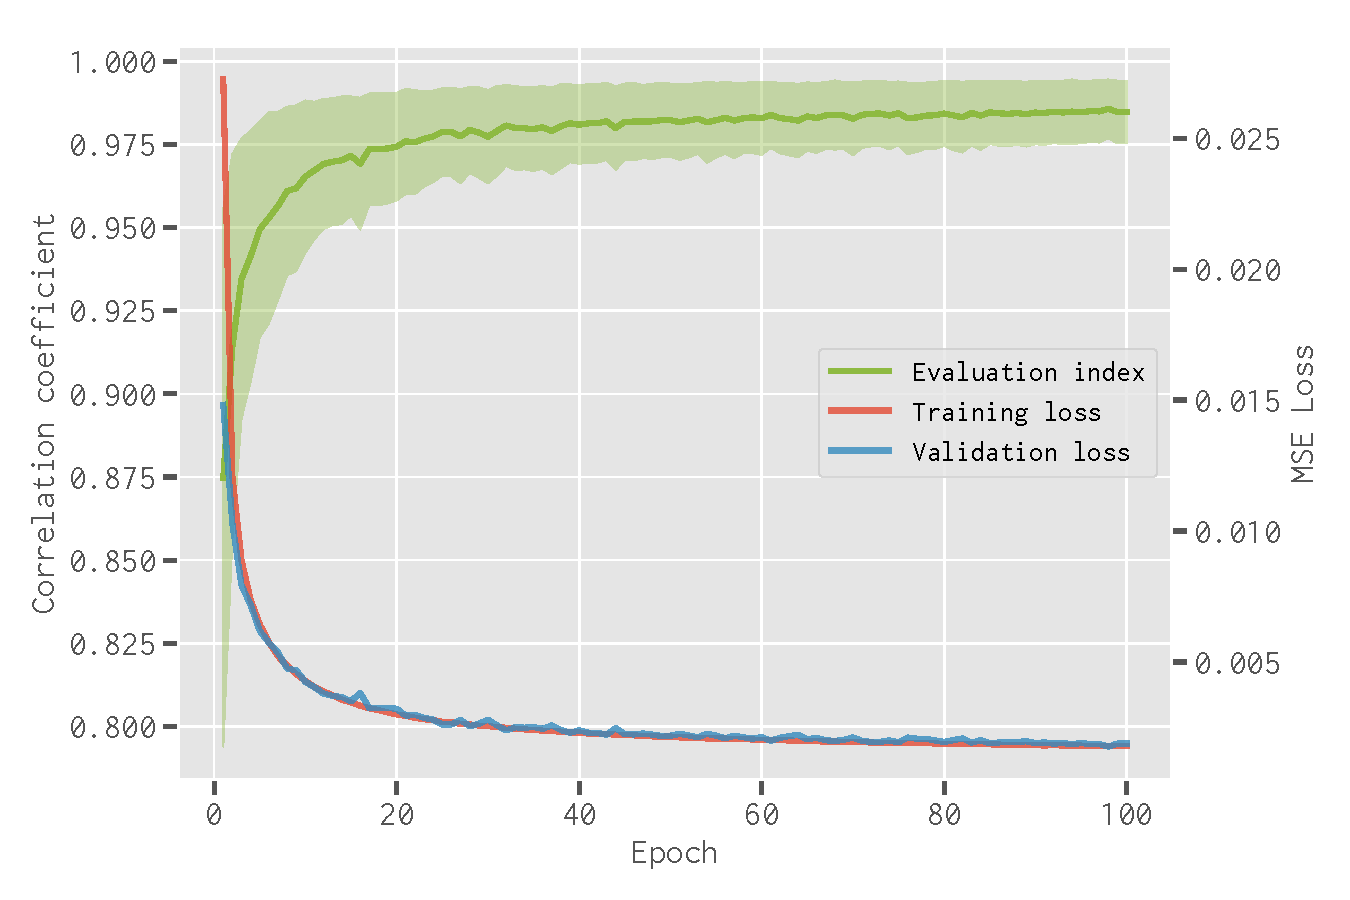
\includegraphics[width=\myfigwidth]{cdae-train}
  \caption{\label{fig:train}%
    The training loss (the red line), validation loss (the blue line),
    and correlation coefficient calculated on the validation set
    $S_{\R{val}}$ (the green line with the shaded region representing
    the standard deviation) during the training of the CDAE.
  }
\end{figure}

\begin{figure}
  \centering
  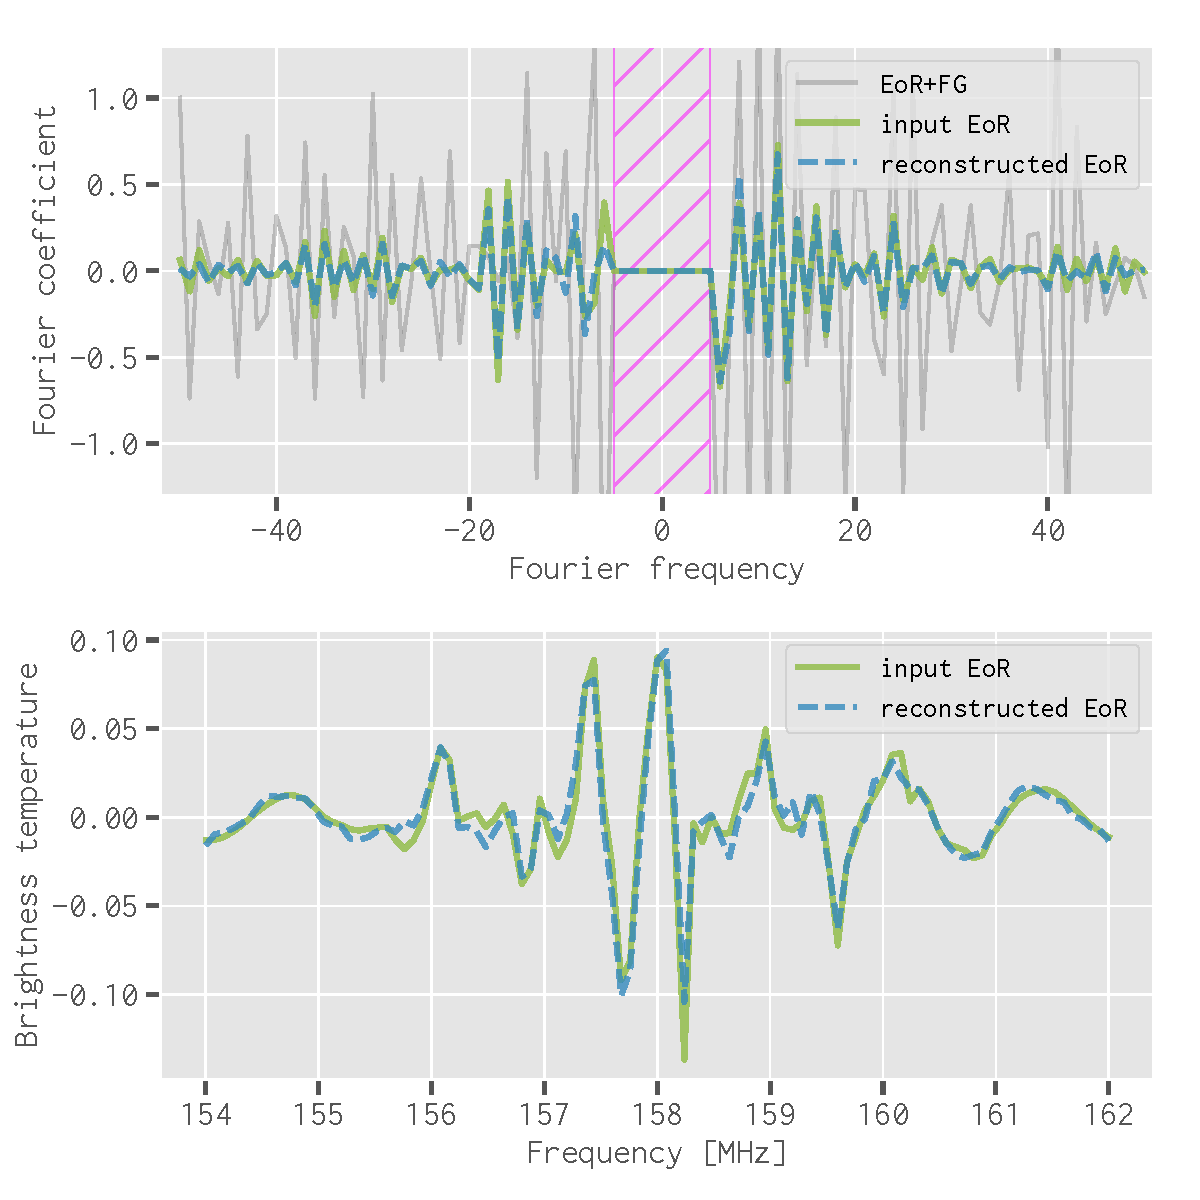
\includegraphics[width=\myfigwidth]{eor-result}
  \caption{\label{fig:result}%
    An example of the EoR signal reconstructed by the trained CDAE for
    one random pixel.
    \textbf{(top)} The input EoR signal (the solid green line) and the
    reconstructed EoR signal (the dashed blue line) in the Fourier domain
    where the CDAE training is performed.
    The grey line represents the corresponding input data that are the
    addition of the EoR signal and the foreground emission.
    The magenta hatched region marks the excised Fourier coefficients
    in data preprocessing.
    \textbf{(bottom)} The input EoR signal (the solid green line) and
    the reconstructed EoR signal (the dashed blue line) transformed back
    to the observing frequency domain.
  }
\end{figure}


%%======================================================================
\section{Discussions}
\label{sec:discussions}

%%----------------------------------------------------------------------
\subsection{Why preprocess dataset with Fourier Transform?}
\label{sec:why-ft}

We have performed another experiment using the same CDAE architecture,
dataset, and data preprocessing steps, except for applying the FT
as depicted in \autoref{sec:preprocessing}.
After training the CDAE in the same way as described in
\autoref{sec:training}, the achieved performance is
$\rho_{\R{noFT}} = \num{0.927 +- 0.051}$, which is smaller than the case
with FT applied, indicating a worse performance with a larger uncertainty.
The losses and the correlation coefficient on the validation set
during the training phase are presented in \autoref{fig:train-noft}.
We also find that the training process is slightly unstable given the
small spikes on the curves of both the training loss and the correlation
coefficient, and the training loss converges slower.
These indicate that it is beneficial to preprocess the
dataset by applying the FT along the frequency dimension, because the FT
renders the EoR signal and the foreground emission more distinguishable
in the Fourier domain, where the fluctuating EoR signal concentrates on
larger Fourier modes while the spectral-smooth foreground emission
distributes mainly on smaller Fourier modes \citep[e.g.,][]{parsons2012}.

\begin{figure}
  \centering
  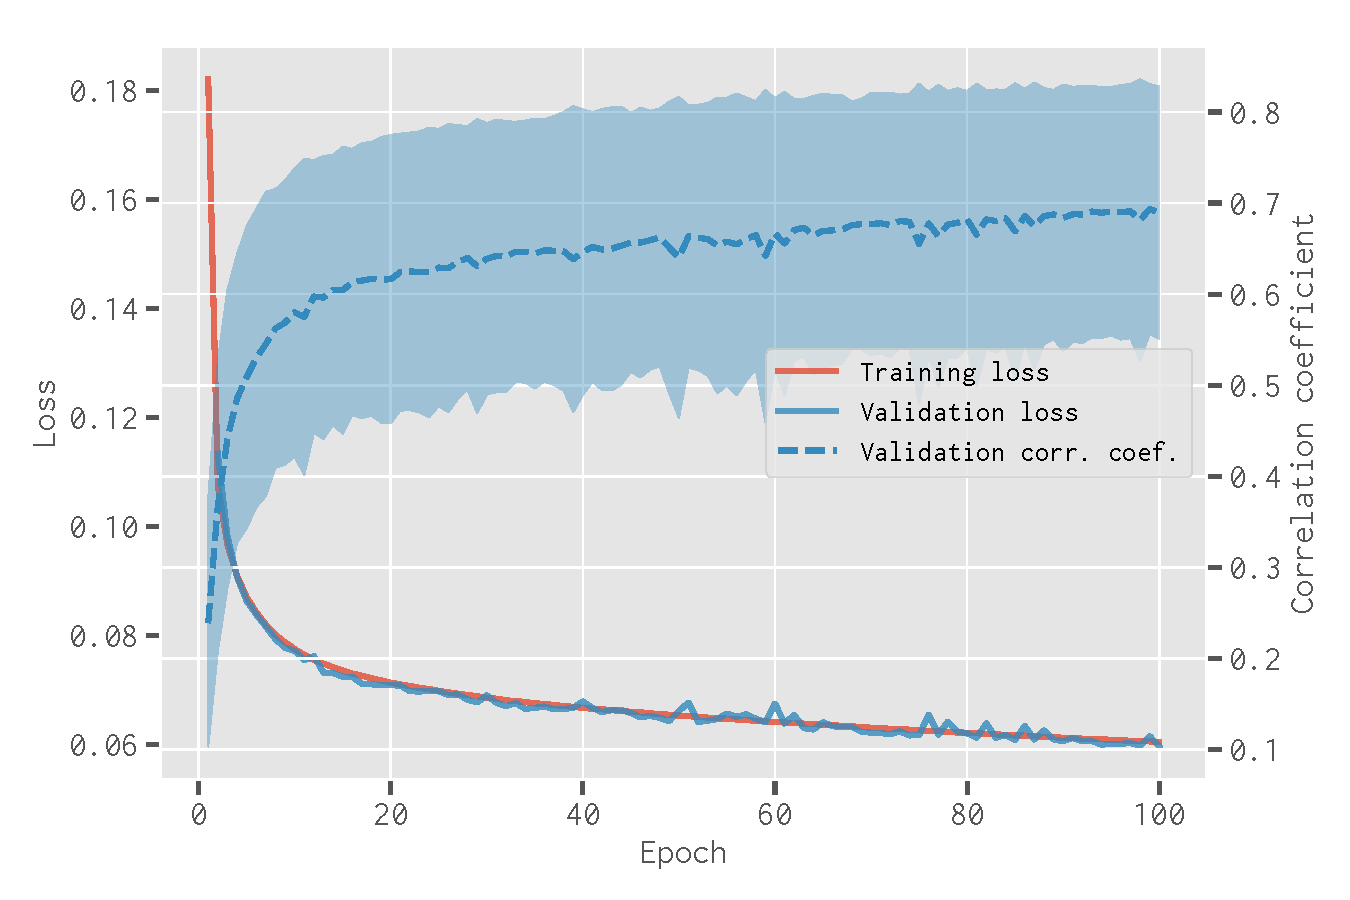
\includegraphics[width=\myfigwidth]{cdae-train-noft}
  \caption{\label{fig:train-noft}%
    Same as \autoref{fig:train} but for the case that the data are
    preprocessed without applying the FT.
  }
\end{figure}


%%----------------------------------------------------------------------
\subsection{Comparing with the standard polynomial fitting method}
\label{sec:polyfit}

In order to further demonstrate the performance of our method, we have
carried out a comparison between our method and the standard polynomial
fitting method \citep[e.g.,][]{wang2006,liu2009ps}.
Using the same image cubes simulated in \autoref{sec:simulation},
a low-degree polynomial is fitted along the frequency dimension for each
pixel in the image cube of the total emission (i.e.,
$C_{\R{tot}} = C_{\R{EoR}} + C_{\R{fg}}$).
Then by subtracting the fitted smooth component, which is regarded as
the foreground emission, the EoR signal is uncovered.
We have tested polynomials of the degree from 2 (quadratic) to
5 (quintic), and find that the quartic polynomial (degree of 4)
can give the best result.
However, the correlation coefficient calculated for the separated EoR
signal in such a case is only $\rho_{\R{poly}} = \num{0.241 +- 0.103}$,
which indicates that the polynomial fitting method
performs poorly in removing the foreground emission.
As illustrated in \autoref{fig:simudata}(b), the frequency-dependent
beam effects cause rapid fluctuations, which can be even stronger than
the EoR signal, on the originally smooth foreground spectrum.
The polynomial fitting method, which can only model the smooth
spectrum, is unable to distinguish these rapid fluctuations from the
EoR signal, hence leading to inferior results.
{\color{cyan}%
On the contrary, given its flexibility and data-driven nature,
the CDAE can learn the features of the EoR signal from the data and
gain superior performance.}


%%======================================================================
\section{Summary}
\label{sec:summary}

The frequency-dependent beam effects of interferometers can cause
complicated fluctuations along the frequency dimension,
which destroy the smoothness of the foreground spectra and prevent
standard foreground removal methods from uncovering the EoR signal.
Given the difficulty in crafting practicable models to overcome the
complicated beam effects, methods that learn from the data seem more
feasible and appealing.
To this end, we have proposed a deep-learning-based method by employing
the CDAE to separate the EoR signal.
The CDAE has been trained on the simulated SKA images and has achieved
excellent performance in separating the EoR signal, demonstrating its
ability to overcome the intricate frequency-dependent beam effects.
In addition, the proposed CDAE has a simple architecture and is easily
extensible, exhibiting the great potential of deep learning methods
to play an important role in the forthcoming EoR experiments.


%%======================================================================
\section*{Acknowledgements}

We would like to thank Jeffrey Hsu for reading the manuscript and
providing suggestions.
This work is supported by
the Ministry of Science and Technology of China
(grant Nos. 2018YFA0404601, 2017YFF0210903),
and the National Natural Science Foundation of China
(grant Nos. 11433002, 11621303, 11835009, 61371147).


%%======================================================================
%% References

\bibliographystyle{mnras}
\bibliography{references}


%%======================================================================
%% Appendix

% \appendix


%%======================================================================
% Don't change these lines
\bsp	% typesetting comment
\label{lastpage}
\end{document}

%% EOF
